\documentclass{ieeetj}
\usepackage{cite}
\usepackage{amsmath,amssymb,amsfonts,amsthm,mathtools}
\usepackage{graphicx,color}
\usepackage{xcolor}
\usepackage{booktabs}
\usepackage{multirow}
\usepackage{url}
\usepackage{bm}
\usepackage{tikz}
\usepackage{hyperref}
\hypersetup{hidelinks=true}
\AtBeginDocument{\definecolor{tmlcncolor}{cmyk}{0.93,0.59,0.15,0.02}\definecolor{NavyBlue}{RGB}{0,86,125}}

% Work around a class-file typo that can print a stray "revised" on page 1.
\makeatletter
\let\@revised\@empty
\makeatother

\usetikzlibrary{arrows.meta,positioning,fit,backgrounds,calc,decorations.pathreplacing}
\def\BibTeX{{\rm B\kern-.05em{\sc i\kern-.025em b}\kern-.08em
    T\kern-.1667em\lower.7ex\hbox{E}\kern-.125emX}}
\def\OJlogo{}
\def\seclogo{}
\def\authorrefmark#1{\ensuremath{^{\textbf{#1}}}}
\newtheorem{theorem}{Theorem}
\newtheorem{corollary}{Corollary}

\begin{document}
\receiveddate{}
\reviseddate{}
\accepteddate{}
\publisheddate{}
\currentdate{}
\doiinfo{}
\markboth{}{Anonymous et al.}
\title{Backbone-Modular Neuro-Symbolic Post-Correction for OCT Denoising via Explicit Predicate Maps and Stable Fuzzy Allocation}
\author{Anonymous Author(s)\authorrefmark{1}}
\affil{\authorrefmark{1} Anonymous Affiliation}
\corresp{Correspondence withheld for double-blind review.}
\authornote{This manuscript is prepared for double-blind review.}

\begin{abstract}
Optical coherence tomography (OCT) denoisers are usually optimized for pixel fidelity, yet clinically important attributes such as layer contrast, boundary definition, and tissue visibility can still degrade after denoising. This paper formulates \emph{post-correction} as a separate technical problem: how to attach a transparent and safety-constrained correction policy to a strong pretrained denoiser without retraining the backbone itself. We present \textbf{CoopNS-OCT}, a backbone-modular neuro-symbolic wrapper composed of a lightweight backbone-specific confidence head, multiplicative and additive correctors, and a differentiable fuzzy negotiator driven by six explicitly defined ground-truth-free predicates. Each predicate is formalized by both a scalar score and a spatial failure map, making the negotiator input reproducible rather than heuristic. We prove that the negotiated allocation map is Lipschitz-stable with respect to predicate perturbations and derive a margin-based lower bound showing when tissue-gated correction improves contrast-to-noise ratio (CNR) despite bounded background leakage. The wrapper adds only 0.168M trainable parameters (about 2.4\% overhead relative to a 7M backbone). On PKU37 and leave-one-out Duke17/Duke2013 evaluation, CoopNS-OCT improves CNR by 10--15\% and boundary sharpness by 2.5--11\%, with sub-dB OOD PSNR trade-offs of 0.25--0.80 dB. The same correction logic transfers across NAFNet, DnCNN, SwinIR, and KBNet after adapting only the confidence head, supporting a reusable post-correction \emph{policy} rather than another OCT backbone.
\end{abstract}

\begin{IEEEkeywords}
Optical coherence tomography, image denoising, neuro-symbolic reasoning, fuzzy logic, interpretable image restoration, modular post-correction, clinical quality assessment.
\end{IEEEkeywords}

%\IEEEspecialpapernotice{(Invited Paper)}

\maketitle

\section{Introduction}
\label{sec:introduction}
\IEEEPARstart{O}{ptical} coherence tomography (OCT) is the dominant non-invasive imaging modality for retinal diagnostics~\cite{huang1991optical}. OCT images are degraded by multiplicative speckle noise~\cite{goodman2007speckle} that obscures layer boundaries, reduces contrast, and limits the reliability of downstream analyses such as layer segmentation~\cite{devalla2018drunet}.

\subsection{Motivation}
Despite rapid progress in deep denoisers~\cite{zhang2017beyond,chen2022simple,liang2021swinir,krull2019noise2void}, most OCT restoration pipelines still optimize denoising as pixel regression. This is often mismatched to clinical use: a backbone can gain PSNR while degrading tissue-background separability, boundary sharpness, or layer visibility. A second problem is interpretability. When a post-processing module changes an OCT scan, clinicians and reviewers should be able to inspect \emph{why} and \emph{where} the correction was applied, rather than treating the adjustment as a black-box residual.

What is missing in the literature is not another denoising block, but a \emph{formal correction interface} between clinical quality criteria and a learned restoration model. The central question of this paper is therefore not ``Can we invent yet another OCT backbone?'' but rather: \emph{Can a clinically meaningful correction policy be expressed as explicit spatial predicates, routed through stable symbolic logic, and attached to strong pretrained denoisers with bounded risk to fidelity?} A convincing answer requires three properties simultaneously: the correction policy must be \emph{explicit}, \emph{stable}, and \emph{safe}. The technical novelty lies in elevating post-correction into a formal optimization object with named predicate interfaces, theorem-backed routing behavior, and safety-gated execution.

\subsection{Contributions}
We propose \textbf{CoopNS-OCT}, a cooperative neuro-symbolic OCT post-correction framework. The paper is positioned as a systems-and-methodology contribution on clinically constrained correction, not as a claim that Sobel edges, fuzzy logic, or uncertainty heads are individually novel. Our contributions are:

\begin{enumerate}
\item \textbf{Backbone-modular cooperative correction} (Section~\ref{sec:cooperative}): a frozen denoising backbone is augmented by a lightweight confidence head, a multiplicative gain corrector, and an additive edge recovery module. The correction layer is shared across backbone families; only the confidence head depends on backbone feature dimensionality. We therefore make the narrower and technically defensible claim of \emph{modularity}, not universal architecture agnosticism.

\item \textbf{Explicit predicate-to-map formalization} (Section~\ref{sec:negotiator}): six ground-truth-free clinical predicates are specified as closed-form score functions together with spatial failure maps. This gives reproducible negotiator inputs rather than qualitative descriptors such as ``edge-to-flat ratio'' or ``vertical consistency'' without formulas.

\item \textbf{Stable symbolic allocation with theorem-backed transfer behavior} (Section~\ref{sec:negotiator}): the negotiator uses differentiable Lukasiewicz logic~\cite{vankrieken2022analyzing} to combine predicate failures into a per-pixel allocation rule. We prove the allocation is Lipschitz-stable with respect to perturbations of the predicate vector, which explains why the same negotiated policy remains well behaved when the backbone is replaced and the calibrated predicate scores shift slightly.

\item \textbf{Safety-gated correction with clinically meaningful guarantees} (Sections~\ref{sec:cnr}--\ref{sec:formal}): tissue-aware gating, bounded perturbation, energy descent, and Pareto-style non-degradation are combined with a margin-based CNR result that makes explicit when the wrapper improves clinically relevant contrast despite bounded background leakage. Cross-dataset leave-one-out (LOO) evaluation on Duke17 and Duke2013 shows consistent gains across four strong learned backbones.
\end{enumerate}

Fig.~\ref{fig:architecture} illustrates the overall architecture. A frozen denoiser produces $\hat{\mathbf{x}}_\text{base}$, a confidence head estimates per-pixel uncertainty, and two lightweight correctors propose multiplicative and additive refinements. A symbolic negotiator then decides where the gain pathway should be active, while safety constraints determine how strongly the corrected candidate may deviate from the backbone output.

\begin{figure*}[t]
\centering
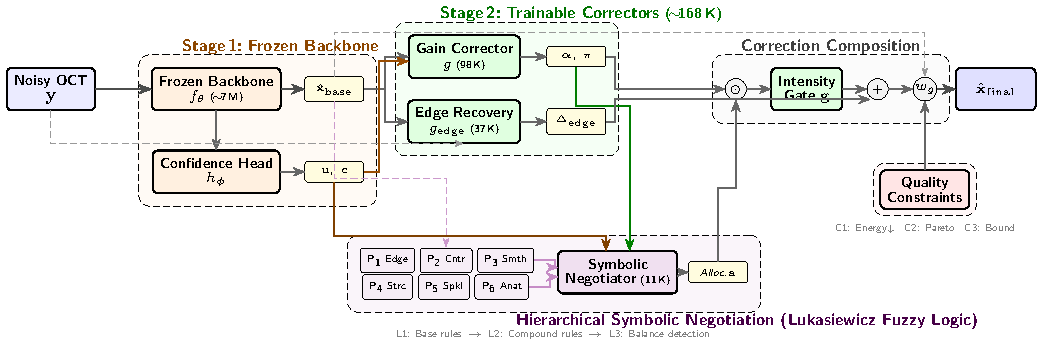
\includegraphics[width=\textwidth]{figures/architecture.pdf}
\caption{Overall architecture of the CoopNS-OCT framework. \textbf{Stage\,1} (orange): a frozen backbone denoiser $f_\theta$ produces the base output $\hat{\mathbf{x}}_{\mathrm{base}}$; a lightweight confidence head $h_\phi$ estimates per-pixel uncertainty $\mathbf{u}$. \textbf{Stage\,2} (green): a multiplicative gain corrector $g_{\mathrm{gain}}$ and an additive edge recovery module $g_{\mathrm{edge}}$ generate corrections guided by uncertainty. The \textbf{hierarchical symbolic negotiator} (violet) evaluates six ground-truth-free clinical predicates ($P_1$--$P_6$) through three levels of differentiable Lukasiewicz fuzzy logic to produce the allocation map $\mathbf{a}$. The \textbf{correction composition} path applies the negotiated gain via an intensity gate, combines it with edge corrections, and blends with the backbone output using weight $w_g$ determined by three quality-preserving constraints (energy descent, Pareto non-degradation, bounded perturbation). The entire correction pipeline adds ${\sim}$168\,K trainable parameters across all stages (${\sim}$2.4\% overhead): gain corrector 98\,K, edge recovery 37\,K, confidence head 22\,K, symbolic negotiator 11\,K.}
\label{fig:architecture}
\end{figure*}

%% =====================================================================
%% II. RELATED WORK
%% =====================================================================
\section{Related Work}
\label{sec:related}

\subsection{OCT Denoising}
Deep learning denoisers span CNN-based methods (DnCNN~\cite{zhang2017beyond}, DRUNET~\cite{devalla2018drunet}), attention architectures (NAFNet~\cite{chen2022simple}, KBNet~\cite{zhang2023kbnet}), and transformers (SwinIR~\cite{liang2021swinir}). Classical approaches (non-local means~\cite{buades2005non}, wavelets~\cite{mayer2012wavelet}) and self-supervised methods (Noise2Void~\cite{krull2019noise2void}) remain relevant. OCT-specific methods---triplet cross-fusion~\cite{geng2022triplet}, sparse representation~\cite{fang2012sparsity,fang2013fast}---address paired-data scarcity but still optimize denoising primarily as fidelity restoration. Automated quality assessment~\cite{wang2019quality} provides quality \emph{measurement} but not quality-driven \emph{correction}. Our framework fills that gap by treating clinically targeted post-correction as a first-class optimization problem attached to, but analytically distinct from, the backbone denoiser.

\subsection{Uncertainty in Medical Image Analysis}
Bayesian dropout~\cite{gal2016dropout}, multi-task uncertainty~\cite{kendall2018multi}, and deep ensembles~\cite{lakshminarayanan2017simple} provide principled frameworks for flagging unreliable predictions in medical imaging. In OCT, uncertainty estimation has been explored for layer segmentation~\cite{devalla2018drunet} and scan quality assessment~\cite{wang2019quality}. However, existing approaches use uncertainty mainly for \emph{detection} rather than \emph{correction}: uncertain regions are identified, but the downstream adjustment mechanism remains absent or purely heuristic. Our framework uses uncertainty as a routing variable inside a constrained correction policy, so uncertainty is not merely reported but operationalized.

\subsection{Neuro-Symbolic AI for Image Processing}
Neuro-symbolic AI~\cite{garcez2023neurosymbolic} integrates neural learning with symbolic reasoning via differentiable fuzzy logic~\cite{vankrieken2022analyzing}, enabling gradient-based optimization of logical rules over continuous-valued inputs. While cooperative architectures---including modular expert systems and multi-objective optimization---share the goal of interpretable decision-making, they have not been used to formalize low-level OCT post-correction as an explicit routing problem over clinically named failure modes. Our Lukasiewicz formulation is therefore not generic interpretability decoration; it is the control law of the wrapper, coupling scalar predicate failures, spatial failure maps, and per-pixel allocation into one auditable decision layer.


%% =====================================================================
%% III. UNCERTAINTY-GUIDED COOPERATIVE CORRECTION
%% =====================================================================
\section{Backbone-Modular Cooperative Correction}
\label{sec:cooperative}

\subsection{Problem Setup}
\label{sec:problem_setup}
Let $\mathbf{y} \in [0,1]^{H \times W}$ denote a noisy OCT B-scan and $\hat{\mathbf{x}}_\text{base} = f_\theta(\mathbf{y})$ the output of a frozen backbone denoiser. While $\hat{\mathbf{x}}_\text{base}$ achieves strong PSNR, it may exhibit clinical deficiencies (over-smoothed boundaries, reduced contrast) because MSE training penalizes all pixel errors equally. Our goal is to produce $\hat{\mathbf{x}}_\text{final}$ that \emph{selectively} improves clinical attributes while preserving fidelity.

\subsection{Backbone Interface and Confidence Estimation}
\label{sec:backbone_uncertainty}
The implementation is \emph{backbone-modular}, not strictly backbone-agnostic. Any frozen denoiser $f_\theta$ can supply the base image $\hat{\mathbf{x}}_\text{base}$, but the confidence head must read a backbone-specific feature tensor $\mathbf{z}$ whose channel count depends on the architecture. The rest of the wrapper---the gain corrector, edge corrector, symbolic negotiator, and safety gates---is shared. We evaluate four representative backbone families: NAFNet~\cite{chen2022simple}, KBNet~\cite{zhang2023kbnet}\footnote{KBNet~\cite{zhang2023kbnet} is a preprint. It is retained because it represents a distinct kernel-basis restoration family; the qualitative conclusions of this paper do not depend on it.}, DnCNN~\cite{zhang2017beyond}, and SwinIR~\cite{liang2021swinir}, each with about 7M frozen parameters. A lightweight confidence head $h_\phi$ produces the per-pixel confidence map
\begin{equation}
\mathbf{c}(\mathbf{y}) = \sigma\!\left(\frac{h_\phi(\mathbf{z}) + b}{\tau}\right) \in [0,1]^{H \times W},
\label{eq:confidence}
\end{equation}
where $\mathbf{z}$ is the backbone-specific feature source in Table~\ref{tab:uncertainty_sources}, $\tau>0$ is a learnable temperature, and $b$ is a learnable bias. The temperature calibrates how sharply the wrapper distinguishes confident from uncertain regions; small $\tau$ produces near-binary routing, while larger $\tau$ distributes correction more softly.

\begin{table}[t]
\centering
\caption{Per-backbone uncertainty feature source. All heads use a two-layer CNN producing a scalar confidence map.}
\label{tab:uncertainty_sources}
\setlength{\tabcolsep}{4pt}
\begin{tabular}{lll}
\toprule
Backbone & Feature source $\mathbf{z}$ & Channels \\
\midrule
NAFNet & First encoder features (enc1) & 40 \\
KBNet & First encoder features (enc1) & 32 \\
DnCNN & Head features (first conv layer) & 228 \\
SwinIR & Shallow features (conv\_first) & 138 \\
\bottomrule
\end{tabular}
\end{table}

\begin{table}[t]
\centering
\caption{Core notation used throughout the pipeline.}
\label{tab:notation}
\setlength{\tabcolsep}{3pt}
\footnotesize
\begin{tabular}{lp{0.60\columnwidth}}
\toprule
Symbol & Meaning \\
\midrule
$y$ & Noisy OCT input B-scan \\
$\hat{x}_{\text{base}}$ & Output of the frozen backbone denoiser \\
$\hat{x}_{\text{corr}}$ & Corrected candidate before safety-gated blending \\
$\hat{x}_{\text{final}}$ & Final output after blending \\
$z$ & Backbone feature tensor used by the confidence head \\
$c,u$ & Confidence and uncertainty maps \\
$\alpha, \Delta_{\mathrm{edge}}$ & Gain and edge correction \\
$s_i,m_i,\tau_i$ & Predicate score, failure map, and decision threshold \\
$f_i$ & Soft predicate-failure activation \\
$\pi,a$ & Potential map and negotiated allocation \\
$w_g$ & Blend weight determined by the safety constraints \\
\bottomrule
\end{tabular}
\end{table}

The uncertainty map is $\mathbf{u}=1-\mathbf{c}$. It is trained jointly with the correctors so that high uncertainty aligns with locations where the wrapper can improve clinical quality and low uncertainty suppresses unnecessary corrections.

\subsection{Corrector Modules}
\label{sec:corrector_modules}
Two complementary modules target different clinical deficiencies: a \emph{multiplicative} gain corrector $g_{\mathrm{gain}}$ for brightness and contrast (scaling with local intensity), and an \emph{additive} edge recovery module $g_\text{edge}$ for boundary sharpness (intensity-independent).

\subsubsection{Multiplicative Gain Corrector}
The gain corrector $g_{\mathrm{gain}}$ operates at quarter resolution ($H/4 \times W/4$), producing a 2-channel gain map---brightness ($\alpha_b$, via ReLU) and contrast ($\alpha_c$, via $\tanh$):
\begin{equation}
\boldsymbol{\alpha} = \alpha_{\max}\!\big(\text{ReLU}(\alpha_b) + \tanh(\alpha_c)\big),
\label{eq:gain_map}
\end{equation}
where $\alpha_{\max} = 0.15$ is the maximum per-pixel gain magnitude, implemented as a learnable soft clamp (sigmoid-scaled within $[0.02, 0.15]$). The correction $\Delta = \boldsymbol{\alpha} \odot \hat{\mathbf{x}}_\text{base}$ is \emph{multiplicative}, matching OCT speckle's multiplicative nature~\cite{goodman2007speckle}---bright tissue receives stronger absolute corrections than dark background.

\subsubsection{Edge Recovery Module}
The edge recovery module $g_\text{edge}$ is a standalone \emph{additive} corrector. A 4-layer CNN processes four complementary channels---intensity-normalized residual $(\mathbf{y} - \hat{\mathbf{x}}_\text{base})/(\hat{\mathbf{x}}_\text{base} + \epsilon)$ revealing noise patterns independent of local brightness, backbone edge magnitude identifying existing boundaries, backbone output providing intensity context, and unsharp mask highlighting fine structures potentially over-smoothed---producing corrections clamped to $[-0.08, +0.08]$ (tighter than the gain bound because additive corrections are scale-invariant). Training uses Sobel-domain supervision:
\begin{equation}
\mathcal{L}_\text{Sobel} = \big\|\nabla\hat{\mathbf{x}}_\text{corr} - \nabla\hat{\mathbf{x}}_\text{base} - (\nabla\mathbf{x}_\text{clean} - \nabla\hat{\mathbf{x}}_\text{base})\big\|^2,
\label{eq:sobel_loss}
\end{equation}
where $\nabla$ denotes the Sobel gradient operator. This module operates independently of the symbolic negotiator, ensuring edge corrections are always applied regardless of gain allocation.

\subsubsection{Potential Assessment}
The gain corrector also estimates a per-pixel \textbf{potential} $\pi \in [0,1]^{H \times W}$:
\begin{equation}
\pi = \sigma\!\big(\text{CNN}(\hat{\mathbf{x}}_\text{base}, \mathbf{m})\big) \cdot \big(0.5 + \mathbf{u}\big),
\label{eq:potential}
\end{equation}
where $\mathbf{m}$ denotes spatial failure maps from clinical predicates (Section~\ref{sec:predicates}). The $(0.5 + \mathbf{u})$ modulation amplifies potential in uncertain regions ($1.5{\times}$) and attenuates it in confident regions ($0.5{\times}$).

\subsection{Cooperative Loss Formulation}
\label{sec:coop_loss}
The corrector should activate where the backbone is uncertain and remain inactive where it is confident. We enforce this by maximizing Pearson correlation between $\mathbf{u}$ and $\pi$:
\begin{equation}
\mathcal{L}_\text{coop} = \frac{1}{2}\,\text{ReLU}\!\big(1 - \rho(\mathbf{u},\, \pi)\big),
\label{eq:coop_loss}
\end{equation}
where $\rho(\cdot,\cdot)$ is computed over all spatial locations. Pearson correlation is used because it is exactly differentiable, affine-invariant, and does not add a window-size hyperparameter. The loss therefore encourages \emph{where} the wrapper acts to match the backbone's uncertainty without overconstraining \emph{how much} it corrects.

\subsection{Correction Composition and Application}
\label{sec:correction_composition}
The corrector outputs are combined through bounding, background suppression, and brightness--contrast separation ($\operatorname{clamp}(x, a, b) = \min(\max(x, a), b)$, $\sigma$ = sigmoid).

\subsubsection{Negotiated Gain Correction}
The raw gain is modulated by the symbolic allocation $\mathbf{a}$ (Section~\ref{sec:negotiator}) and per-pixel strength $\lambda$ (sigmoid network), then clamped:
\begin{equation}
\boldsymbol{\delta} = \operatorname{clamp}\!\Big(\mathbf{a} \odot \lambda \odot \Delta,\; -0.20,\; 0.20\Big).
\label{eq:composition}
\end{equation}
The bounds $\pm 0.20$ accommodate the bipolar contrast channel and provide the worst-case guarantee in Section~\ref{sec:formal}.

\subsubsection{Intensity Gating}
A scanner-agnostic gate suppresses corrections in background regions:
\begin{equation}
\mathbf{g}(i) = \sigma\!\big(20 \cdot (\hat{x}_{\text{base},i} - q_{0.15})\big),
\label{eq:intensity_gate}
\end{equation}
where $q_{0.15}$ is the 15th intensity percentile of $\hat{\mathbf{x}}_{\text{base}}$, a per-image adaptive threshold capturing vitreous and sub-RPE dark regions across scanners. Background noise is further reduced by a masked $3{\times}3$ mean filter:
\begin{equation}
\hat{x}_i^\text{bg} = \frac{\sum_{j \in \mathcal{N}_i} \hat{x}_j \cdot b_j^\text{erode}}{\sum_{j \in \mathcal{N}_i} b_j^\text{erode}},
\label{eq:bg_smooth}
\end{equation}
where $\mathbf{b}^\text{erode}$ is the background mask eroded by 2 pixels to prevent blur from leaking into tissue boundaries. (Detailed derivations of the background smoothing and intensity gating operations are provided in the supplementary material.)

\subsubsection{Final Composition}
The gain-corrected intermediate separates brightness (smoothed) from contrast adjustments:
\begin{equation}
\hat{\mathbf{x}}_\text{mult} = \hat{\mathbf{x}}_\text{base} + \mathbf{g} \odot \text{smooth}(\text{ReLU}(\boldsymbol{\delta})) + \mathbf{g} \odot (\boldsymbol{\delta} - \text{ReLU}(\boldsymbol{\delta})),
\label{eq:xmult}
\end{equation}
The corrected output combines gain and edge corrections:
\begin{equation}
\hat{\mathbf{x}}_\text{corr} = \operatorname{clamp}\!\big(\hat{\mathbf{x}}_\text{mult} + \mathbf{g} \odot \Delta_\text{edge},\; 0,\; 1\big).
\label{eq:final}
\end{equation}
The remaining question is how to determine $\mathbf{a}$: \emph{when}, \emph{where}, and \emph{how much} the gain corrector should contribute.

%% =====================================================================
%% IV. HIERARCHICAL SYMBOLIC NEGOTIATION
%% =====================================================================
\section{Hierarchical Symbolic Negotiation}
\label{sec:negotiator}

Rather than learning the allocation $\mathbf{a}$ in Eq.~\eqref{eq:composition} as an opaque attention map, we compute it through a three-level symbolic reasoner. The key point for this submission is reproducibility: the negotiator does not consume vaguely described ``clinical features,'' but six explicitly defined predicate scores together with six spatial failure maps.

\subsection{Ground-Truth-Free Clinical Predicates}
\label{sec:predicates}
Let $x=\hat{\mathbf{x}}_\text{base}$, $y$ be the noisy OCT input, $e(x)=\sqrt{(S_x*x)^2+(S_y*x)^2}$ the Sobel edge magnitude, $\theta(x)=\operatorname{atan2}(S_y*x,S_x*x)$ the local edge angle, and $\mu_k(\cdot),\sigma_k(\cdot)$ the local mean and standard deviation in a $k\times k$ window. In Table~\ref{tab:predicates}, $\operatorname{sigm}(t)$ is the logistic sigmoid, $e_{\max}=\max e(x)$, $\langle a,b\rangle=\sum_p a_p b_p$, $\|a\|_1=\sum_p |a_p|$, $\operatorname{mean}_w$ averages laterally, $\nabla_z$ and $\operatorname{Var}_z$ act along axial depth, and $\operatorname{clip}(u,0,1)$, $[u]_{[0,1]}$, and $\operatorname{ReLU}(u)$ have their standard meanings. Each predicate outputs a scalar score $s_i\in[0,1]$ summarizing image-level quality and a failure map $\mathbf{m}_i\in[0,1]^{H\times W}$ localizing where correction should be encouraged. Thresholds $\tau_i$ are calibrated during training and then fixed at inference.

\begin{table*}[t]
\centering
\caption{Ground-truth-free predicates used by the symbolic negotiator. For each predicate, the table lists its clinical role, image-level score, and pixel-level failure map; larger $\mathbf{m}_i$ means stronger evidence that the corresponding property is locally unsatisfied. Detailed subterm definitions follow immediately below. Here $\bar e=\operatorname{mean}(e(x))$, $b_e=\mathbf{1}[e(x)>\bar e]$, $v(z)=\operatorname{mean}_w z$ is a depth profile, $\rho_h$ is 1-pixel horizontal autocorrelation, and $\operatorname{Var}_k$ is local variance over a $k\times k$ window.}
\label{tab:predicates}
\setlength{\tabcolsep}{3pt}
\footnotesize
\begin{tabular}{cp{0.18\textwidth}p{0.33\textwidth}p{0.28\textwidth}c}
\toprule
$P_i$ & Clinical role & Aggregate score $s_i$ & Failure map $\mathbf{m}_i$ & $\tau_i$ \\
\midrule
$P_1$ & Edge continuity &
$0.4\,c_{\text{cont}}+0.3\,c_{\text{efr}}+0.3\,c_{\text{ang}}$ &
$(1-\tilde e)(1-b_e)$, \ $\tilde e=e(x)/(e_{\max}+\varepsilon)$ &
0.6 \\
$P_2$ & Local contrast recovery &
$0.20\,s_{\text{range}}+0.35\,s_{\text{cnr}}+0.20\,s_{\text{var}}+0.25\,s_{\text{cov}}$ &
$[\operatorname{ReLU}(\bar\sigma-\sigma_9(x))/(\bar\sigma+\varepsilon)+0.3\,\mathbf{1}[\sigma_9(x)<0.01]]_{[0,1]}$ &
0.5 \\
$P_3$ & Flat-region smoothness &
$0.6\,q_{\text{var}}+0.4\,q_{\text{res}}$ &
$F \odot \sigma_5(x)/(\max \sigma_5(x)+\varepsilon)$ &
0.75 \\
$P_4$ & Structural coherence &
$0.4\,s_{\text{self}}+0.3\,s_{\text{reg}}+0.3\,s_{\text{vert}}$ &
$e(e(x))/(\max e(e(x))+\varepsilon)$ &
0.5 \\
$P_5$ & Speckle conformity &
$0.7\,\operatorname{mean}(\exp(-|cv-cv^\star|/0.15))+0.3\,\exp(-5|\rho_h(z)|)$ &
$1-\exp(-|cv-cv^\star|/0.15)$ &
0.3 \\
$P_6$ & Layer visibility &
$0.4\,s_{\text{clr}}+0.3\,s_{\text{dep}}+0.3\,s_{\text{smo}}$ &
$\operatorname{Var}_7(e(x))/(\max \operatorname{Var}_7(e(x))+\varepsilon)$ &
0.7 \\
\bottomrule
\end{tabular}
\end{table*}

{\footnotesize
\noindent\textbf{Expanded subterms in Table~\ref{tab:predicates}.}
\textbf{$P_1$:}
$c_{\text{cont}}=\langle\operatorname{erode}(\operatorname{dilate}(b_e)),b_e\rangle/(\|b_e\|_1+\varepsilon)$,
$c_{\text{efr}}=\exp(-5|r_e-0.2|)$ with
$r_e=\|\mathbf{1}[e(x)>1.5\bar e]\|_1/(\|\mathbf{1}[e(x)<0.5\bar e]\|_1+\varepsilon)$,
and $c_{\text{ang}}=\exp(-2\,\operatorname{mean}(\sigma_5(\theta(x))))$.
\textbf{$P_2$:}
$s_{\text{range}}=\operatorname{sigm}(10(\Delta_r-0.3))$, $\Delta_r=\max(x)-\min(x)$;
$s_{\text{cnr}}=\operatorname{sigm}(15(\bar\sigma-0.05))$, $\bar\sigma=\operatorname{mean}(\sigma_9(x))$;
$s_{\text{var}}=\max(0.2,\operatorname{sigm}(-20(v_\sigma-0.02)+2))$, $v_\sigma=\operatorname{Var}(\sigma_9(x))$;
$s_{\text{cov}}=\operatorname{sigm}(5(\gamma-0.4))$, $\gamma=\operatorname{mean}(\mathbf{1}[\sigma_9(x)>0.3\bar\sigma])$.
\textbf{$P_3$:}
$F=\mathbf{1}[e(x)<0.3\bar e]$,
$q_{\text{var}}=1-\langle F,\sigma_5(x)/(\sigma_5(y)+\varepsilon)\rangle/(\|F\|_1+\varepsilon)$,
and $q_{\text{res}}=\exp(-5\,\operatorname{mean}|y-x|)$.
\textbf{$P_4$:}
$s_{\text{self}}$ is the average Pearson correlation between $x$ and shifts $(0,2)$, $(2,0)$, and $(2,2)$;
$s_{\text{reg}}=\exp(-12\,\operatorname{mean}(e(e(x))))$;
$s_{\text{vert}}=\operatorname{clip}(\max |\nabla_z v(x)|/(8\,\operatorname{mean}|\nabla_z v(x)|),0,1)$.
\textbf{$P_5$:}
$z=\log(y+\varepsilon)-\log(x+\varepsilon)$,
$cv=\sigma_{15}(|z|)/(\mu_{15}(|z|)+\varepsilon)$,
and $cv^\star(d)$, where $d$ is the axial depth index, is the depth-wise Gamma-K target coefficient of variation used by the implementation.
\textbf{$P_6$:}
$s_{\text{clr}}=\operatorname{mean}(\operatorname{clip}(\max |\nabla_z v(x)|/(10\,\operatorname{mean}|\nabla_z v(x)|),0,1))$,
$s_{\text{dep}}=\operatorname{clip}(20\,\operatorname{Var}(v(x)),0,1)$,
and $s_{\text{smo}}=1-\operatorname{clip}(10\,\operatorname{mean}(\operatorname{Var}_z(\operatorname{mean}_w e(x))),0,1)$.

These are the implemented predicates. The maps $\mathbf{m}_i$ are the spatial quantities consumed by the negotiator and potential head, while the scores $s_i$ drive the rule activations.
}

\subsection{Differentiable Fuzzy Logic}
\label{sec:fuzzy}
To compose predicate scores into allocation decisions through differentiable logical rules, we adopt Lukasiewicz fuzzy logic~\cite{vankrieken2022analyzing}. Compared with product and minimum-based rules, the Lukasiewicz connectives are piecewise-linear and have bounded slopes, which is useful when the logic layer is embedded in a gradient-trained correction pipeline. The operators are
\begin{align*}
\text{AND}(a,b) &= \max(0,\; a + b - 1), \\
\text{OR}(a,b) &= \min(1,\; a + b), \\
\text{NOT}(a) &= 1 - a, \\
\text{XOR}(a,b) &= |a - b|.
\end{align*}
Each predicate score is first converted to a soft failure signal:
\begin{equation}
f_i = \sigma\!\big(\kappa \cdot (\tau_i - s_i)\big),
\label{eq:soft_failure}
\end{equation}
where $\kappa=10$ controls the sharpness of the score-to-failure conversion.

\subsection{Three-Level Hierarchical Reasoning}
The symbolic reasoner composes the six failure signals into correction decisions through three levels of abstraction.

\textbf{Level 1:} each predicate score is converted to its soft failure value $f_i$ using Eq.~\eqref{eq:soft_failure}.

\textbf{Level 2:} clinically motivated conjunctions amplify multi-factor failures:
\begin{align}
r_\text{ec} &= 1.5 \cdot \text{AND}(f_\text{edge}, f_\text{contrast}), \label{eq:compound1} \\
r_\text{comp} &= 2.0 \cdot \text{AND}\!\big(\text{OR}(f_\text{edge}, f_\text{contrast}),\; f_\text{struct}\big). \label{eq:compound2}
\end{align}
Rule $r_\text{ec}$ detects simultaneous edge and contrast failure, while $r_\text{comp}$ detects a broader structural breakdown accompanied by either edge or contrast weakness.

\textbf{Level 3:} a balance detector suppresses gain correction when the image is already smooth and only edge repair is still needed:
\begin{equation}
c_\text{ge} = \text{XOR}\!\big(\text{NOT}(f_\text{smooth}),\, f_\text{edge}\big).
\label{eq:balance}
\end{equation}

\subsection{Corrector Allocation}
The per-pixel allocation is
\begin{equation}
\begin{aligned}
\mathbf{a} ={}&
\underbrace{\pi \odot \mathbf{c}}_{\text{cooperation}} \odot
\underbrace{\big(w_{\text{base}} + r_{\text{ec}}\mathbf{m}_{\text{contrast}}
+ r_{\text{comp}}\mathbf{m}_{\text{struct}}\big)}_{\text{specialization}} \\
&\odot \underbrace{(1 - c_{\text{ge}})}_{\text{balance}}
\end{aligned}
\label{eq:allocation}
\end{equation}
where $w_\text{base}$ is a learned scalar and $\mathbf{m}_\text{contrast},\mathbf{m}_\text{struct}$ come from $P_2$ and $P_4$. Each pixel-level gain activation can therefore be traced to confidence, potential, and named predicate failures. The next theorem makes precise that this routing rule is stable with respect to small shifts in the predicate failures.

\begin{theorem}[Allocation stability]
\label{thm:allocation_stability}
Fix any pixel $p$ and define $a_p(f)$ by Eq.~\eqref{eq:allocation}, where $f=(f_\text{edge},f_\text{contrast},f_\text{smooth},f_\text{struct})\in[0,1]^4$. Hold $\pi_p$, $c_p$, $m_{\text{contrast},p}$, $m_{\text{struct},p}$, and $w_\text{base}$ fixed. Then for any $f,f'\in[0,1]^4$,
\begin{equation}
|a_p(f)-a_p(f')| \le \pi_p c_p \bigl(9 + 2(w_\text{base}+3.5)\bigr)\,\|f-f'\|_\infty.
\label{eq:allocation_stability}
\end{equation}
\end{theorem}
\begin{proof}
Lukasiewicz AND and OR are 1-Lipschitz in each argument. Hence
$\text{AND}(f_\text{edge},f_\text{contrast})$ and
$\text{OR}(f_\text{edge},f_\text{contrast})$ are both $2$-Lipschitz in $\|\cdot\|_\infty$, so
$r_\text{ec}=1.5\cdot \text{AND}(f_\text{edge},f_\text{contrast})$ is $3$-Lipschitz. For
$h(f)=\text{AND}(\text{OR}(f_\text{edge},f_\text{contrast}),f_\text{struct})$,
$|h(f)-h(f')|
\le |\text{OR}(f_\text{edge},f_\text{contrast})-\text{OR}(f'_\text{edge},f'_\text{contrast})|
+ |f_\text{struct}-f'_\text{struct}|
\le 3\|f-f'\|_\infty$,
so $r_\text{comp}=2h$ is $6$-Lipschitz. Therefore the specialization factor
$A(f)=w_\text{base}+r_\text{ec}m_{\text{contrast},p}+r_\text{comp}m_{\text{struct},p}$
is $(3+6)=9$-Lipschitz and bounded above by
$M:=w_\text{base}+1.5+2=w_\text{base}+3.5$.
The balance factor $B(f)=1-\text{XOR}(1-f_\text{smooth},f_\text{edge})$ is $2$-Lipschitz and satisfies $0\le B(f)\le 1$.
Since $a_p(f)=\pi_p c_p A(f)B(f)$, the product rule gives
\begin{align*}
|A(f)B(f)-A(f')B(f')|
&\le |A(f)-A(f')|\,|B(f)| \\
&\quad + |A(f')|\,|B(f)-B(f')| \\
&\le |A(f)-A(f')| \\
&\quad + M|B(f)-B(f')|,
\end{align*}
Multiplying by $\pi_pc_p$ yields Eq.~\eqref{eq:allocation_stability}.
\end{proof}

\begin{corollary}[Backbone-modular transfer]
If replacing one backbone by another changes the calibrated failure vector by at most $\varepsilon$ in $\|\cdot\|_\infty$ at pixel $p$, while $\pi_p$, $c_p$, $m_{\text{contrast},p}$, and $m_{\text{struct},p}$ are held fixed, then the negotiated allocation changes by at most $\pi_p c_p (9+2(w_\text{base}+3.5))\varepsilon$. Thus the symbolic routing component is stable under small backbone-dependent calibration shifts in the predicate scores. This corollary is a local stability statement for the routing rule, not a global performance guarantee across backbones.
\end{corollary}

%% =====================================================================
%% V. REGION-AWARE CNR-PRESERVING CORRECTION
%% =====================================================================
\section{Region-Aware CNR-Preserving Correction}
\label{sec:cnr}

This section addresses \emph{how much} correction is safe. The gain pathway is designed to improve clinically useful contrast while the safety layer keeps the corrected image anchored to the backbone when the symbolic evidence is weak.

\subsection{CNR-Preserving Design}
\label{sec:cnr_design}
CNR $=(\mu_\mathcal{T}-\mu_\mathcal{B})/\sigma_\mathcal{B}$ is the most important clinical quantity targeted by the wrapper~\cite{rodriguez2020generalized}. Three design choices act in its favor: \emph{(i)} intensity gating in Eq.~\eqref{eq:intensity_gate} suppresses background corrections, \emph{(ii)} the brightness branch is non-negative, and \emph{(iii)} background smoothing in Eq.~\eqref{eq:bg_smooth} reduces $\sigma_\mathcal{B}$ rather than amplifying it.

\subsection{Quality-Preserving Constraints}
\label{sec:formal}
Beyond CNR, we require holistic quality assurance. Three constraints---at different granularity levels---are enforced softly during training and checked at inference.

\textbf{Constraint 1: Energy descent} (aggregate). A scalar energy summarizes overall clinical quality:
\begin{equation}
E(\hat{\mathbf{x}}) = \underbrace{1 - \frac{1}{6}\sum_{i=1}^{6} s_i(\hat{\mathbf{x}})}_{\text{mean quality deficit}} + \underbrace{0.1 \sum_{i=1}^{6} \max\big(0, 0.5 - s_i(\hat{\mathbf{x}})\big)}_{\text{critical-failure penalty}}
\label{eq:energy}
\end{equation}
Lower energy $=$ better quality. The penalty term (weight $0.1$) nudges the system away from critically low individual scores. We require $E(\hat{\mathbf{x}}_\text{final}) \leq E(\hat{\mathbf{x}}_\text{base}) + \delta_E$ with $\delta_E = 0.05$ (at most 5\% aggregate quality reduction).

\textbf{Constraint 2: Multi-objective non-degradation} (per-predicate). A relaxed Pareto condition prevents improving one predicate while degrading others: $\exists\, i: s_i^\text{corr} - s_i^\text{base} > 0.01$ and $\forall\, j: s_j^\text{corr} - s_j^\text{base} > -0.05$. Both must hold simultaneously ($0.01$ threshold exceeds floating-point noise; $-0.05$ tolerance allows at most 5\% per-predicate regression).

\textbf{Constraint 3: Bounded perturbation} (pixel-level):
\begin{equation}
\frac{\|\hat{\mathbf{x}}_\text{corr} - \hat{\mathbf{x}}_\text{base}\|_2}{\|\hat{\mathbf{x}}_\text{base}\|_2} < L, \quad L = 0.3.
\label{eq:bounded_perturbation}
\end{equation}
The bound $L = 0.3$ (30\% relative $\ell_2$ perturbation) is motivated by the combined per-pixel clamps of the gain and edge pathways ($\pm 0.20$ and $\pm 0.08$) together with typical denoised OCT intensities (${\sim}$0.3--0.5), and is retained as a conservative global limit. This is the strictest of the three constraints: while Constraints~1 and~2 operate on aggregate and per-predicate scores, Constraint~3 directly limits pixel-level change magnitude.

\textbf{Constraint-gated blending.} The number of satisfied constraints controls the blending:
\begin{equation}
\hat{\mathbf{x}}_\text{final} = (1 - w_g) \cdot \hat{\mathbf{x}}_\text{base} + w_g \cdot \hat{\mathbf{x}}_\text{corr},
\label{eq:blend}
\end{equation}
where $w_g = 0.1 + 0.85 \cdot (n_\text{pass}/3)$ and $n_\text{pass} \in \{0,1,2,3\}$, yielding $w_g \in \{0.10, 0.38, 0.67, 0.95\}$. The framework trusts its corrections in proportion to how many safety checks pass. The floor 0.10 preserves gradient signal during early training; the ceiling 0.95 retains a 5\% backbone anchor (selected via grid search on PKU37 validation).

\subsubsection{Stability and CNR Guarantee}

From Eq.~\eqref{eq:blend}, the per-pixel deviation is $w_g(\hat{x}_{\mathrm{corr},i}-\hat{x}_{\mathrm{base},i})$. With the gain and edge clamps combined into $\epsilon=\epsilon_{\mathrm{gain}}+\epsilon_{\mathrm{edge}}=0.20+0.08=0.28$, the final output always satisfies
\begin{equation}
|\hat{x}_{\mathrm{final},i}-\hat{x}_{\mathrm{base},i}| \le w_g\epsilon.
\label{eq:pixel_bound}
\end{equation}
Thus the worst-case perturbation is $0.27$ when all constraints pass and only $0.03$ when none pass.

\begin{corollary}[Margin-based CNR improvement]
\label{cor:cnr}
Let $\eta_\mathcal{T}:=\mu_\mathcal{T}^{\text{corr}}-\mu_\mathcal{T}^{\text{base}}\ge 0$ and assume $\mu_\mathcal{B}^{\text{corr}}-\mu_\mathcal{B}^{\text{base}}\le \eta_\mathcal{B}$. If $\sigma_\mathcal{B}^{\text{corr}}\le \sigma_\mathcal{B}^{\text{base}}$, then
\begin{equation}
\mathrm{CNR}_{\mathrm{final}} \ge \frac{(\mu_\mathcal{T}^{\text{base}}-\mu_\mathcal{B}^{\text{base}}) + w_g(\eta_\mathcal{T}-\eta_\mathcal{B})}{\sigma_\mathcal{B}^{\text{base}}}.
\label{eq:cnr_lb}
\end{equation}
Consequently, whenever $\eta_\mathcal{T}>\eta_\mathcal{B}$, the wrapper cannot decrease CNR.
\end{corollary}
\begin{proof}
By convex blending,
$\mu_\mathcal{T}^{\text{final}}=(1-w_g)\mu_\mathcal{T}^{\text{base}}+w_g\mu_\mathcal{T}^{\text{corr}}$
and similarly for $\mu_\mathcal{B}^{\text{final}}$. Hence
\[
\mu_\mathcal{T}^{\text{final}}-\mu_\mathcal{B}^{\text{final}}
\ge (\mu_\mathcal{T}^{\text{base}}-\mu_\mathcal{B}^{\text{base}})
+ w_g(\eta_\mathcal{T}-\eta_\mathcal{B}).
\]
For the denominator, over background pixels
$x_\mathcal{B}^{\text{final}}=(1-w_g)x_\mathcal{B}^{\text{base}}+w_g x_\mathcal{B}^{\text{corr}}$,
so by Minkowski's inequality applied to centered random variables,
\[
\sigma_\mathcal{B}^{\text{final}}
\le (1-w_g)\sigma_\mathcal{B}^{\text{base}} + w_g \sigma_\mathcal{B}^{\text{corr}}
\le \sigma_\mathcal{B}^{\text{base}}.
\]
Dividing the numerator lower bound by the denominator upper bound gives Eq.~\eqref{eq:cnr_lb}. Because $w_g\in\{0.10,0.38,0.67,0.95\}$, we have $w_g>0$; therefore if $\eta_\mathcal{T}>\eta_\mathcal{B}$, the lower bound in Eq.~\eqref{eq:cnr_lb} is at least the baseline CNR, so the wrapper cannot decrease CNR (under the background-variance condition $\sigma_\mathcal{B}^{\text{corr}}\le \sigma_\mathcal{B}^{\text{base}}$ above).
\end{proof}

In the actual implementation, $\eta_\mathcal{B}$ is kept small by the percentile gate in Eq.~\eqref{eq:intensity_gate}, while the background smoothing of Eq.~\eqref{eq:bg_smooth} pushes $\sigma_\mathcal{B}^{\text{corr}}$ downward. The empirical results in Section~\ref{sec:experiments} are consistent with this design: the mean PSNR changes remain within the bound implied by Eq.~\eqref{eq:pixel_bound}, while CNR improves in all backbone--dataset combinations reported in Table~\ref{tab:duke17_loo}.

%% =====================================================================
%% VI. EXPERIMENTAL RESULTS
%% =====================================================================
\section{Experimental Results}
\label{sec:experiments}

\subsection{Setup}
\label{sec:setup}

\subsubsection{Architecture and Training}
Our system adds ${\sim}$168K trainable parameters to a frozen backbone (${\sim}$7M params), broken down as: gain corrector 98K, edge recovery module 37K, confidence head 22K, and symbolic negotiator 11K. We evaluate four backbones: NAFNet~\cite{chen2022simple}, KBNet~\cite{zhang2023kbnet}, DnCNN~\cite{zhang2017beyond}, and SwinIR~\cite{liang2021swinir}.

Training follows two stages. \textbf{Stage~1:} the backbone is pre-trained on the PKU37 training split with MSE loss for 100 epochs using Adam~\cite{kingma2015adam} ($\text{lr} = 2\!\times\!10^{-4}$, cosine decay), then frozen. \textbf{Stage~2:} all corrector modules are trained jointly for 15 epochs with a composite loss:
\begin{equation}
\mathcal{L} = \mathcal{L}_\text{fidelity} + w_c\,\mathcal{L}_\text{clinical} + w_p\,\mathcal{L}_\text{pred} + w_o\,\mathcal{L}_\text{coop} + w_s\,\mathcal{L}_\text{Sobel},
\label{eq:total_loss}
\end{equation}
The individual terms are:
\begin{itemize}
\item $\mathcal{L}_\text{fidelity}$: pixel-level guard combining MSE and structural similarity index (SSIM), $\mathcal{L}_\text{fidelity} = \|\hat{\mathbf{x}}_\text{final} - \mathbf{x}_\text{clean}\|^2 + 1 - \text{SSIM}(\hat{\mathbf{x}}_\text{final}, \mathbf{x}_\text{clean})$~\cite{wang2004image};
\item $\mathcal{L}_\text{clinical}$: log-ratio clinical improvement loss, $\mathcal{L}_\text{clinical} = -\log(\text{CNR}_\text{corr}/\text{CNR}_\text{base}) - \log(\text{TCI}_\text{corr}/\text{TCI}_\text{base})$, which operates in log-space for scale invariance;
\item $\mathcal{L}_\text{pred} = \sum_{i=1}^{6}(s_i - \tau_i)^2$: regresses predicate scores toward their thresholds to calibrate the negotiator;
\item $\mathcal{L}_\text{coop}$: cooperation loss (Eq.~\eqref{eq:coop_loss});
\item $\mathcal{L}_\text{Sobel}$: edge recovery supervision (Eq.~\eqref{eq:sobel_loss}).
\end{itemize}
Weights are $w_c = 4.0$, $w_p = 1.0$, $w_o = 1.0$, $w_s = 1.0$. The clinical loss weight $w_c = 4.0$ compensates for the smaller magnitude of log-ratio terms relative to pixel-level fidelity, selected via grid search over $\{1, 2, 4, 8\}$ on PKU37 validation. We use AdamW~\cite{loshchilov2019decoupled} ($\text{lr} = 5\!\times\!10^{-4}$, weight decay $10^{-4}$) with mixed-precision training, $96\times 96$ random crops, and batch size~4.

\subsubsection{Datasets}
\label{sec:datasets}

We evaluate on three retinal OCT datasets from different scanners (Table~\ref{tab:datasets}). Paired noisy--clean OCT data requires multi-frame averaging under strict fixation, making large-scale collection impractical~\cite{geng2022triplet}; the datasets below represent the largest publicly available paired OCT benchmarks. \textbf{PKU37}~\cite{geng2022triplet} provides 37 cross-sections ($640{\times}640$) from a custom spectral-domain OCT (SD-OCT) with 50-frame averaged references; we split by clean image identity (27/5/5) yielding 1388/173/173 train/val/test pairs. \textbf{Duke17}~\cite{fang2012sparsity} (named after 16 paired B-scans plus one reserved for protocol validation) contains 16 paired B-scans (${\sim}970{\times}520$) from a clinical SD-OCT at Duke University; we evaluate using leave-one-out (LOO) cross-validation (16 folds), training on 15 images and testing on the held-out image. \textbf{Duke2013}~\cite{fang2013fast} provides 18 synthetic volumes ($900{\times}450$) with controlled degradation.

\begin{table}[t]
\centering
\caption{Datasets. PKU37 is the in-distribution (ID) domain; Duke17 is the primary cross-dataset benchmark with LOO evaluation.}
\label{tab:datasets}
\resizebox{\columnwidth}{!}{%
\begin{tabular}{lllcl}
\toprule
Dataset & Scanner & Size & $N$ & Role \\
\midrule
PKU37 \cite{geng2022triplet} & SD-OCT (PKU) & $640^2$ & 1388/173/173 & ID \\
Duke17 \cite{fang2012sparsity} & SD-OCT (Duke) & $970{\times}520$ & 16 & Out-of-distribution (OOD) LOO \\
Duke2013 \cite{fang2013fast} & Synthetic & $900{\times}450$ & 18 & OOD \\
\bottomrule
\end{tabular}}
\end{table}

\subsubsection{Baselines}

The primary baselines are four strong learned denoisers scaled to about 7M parameters: NAFNet~\cite{chen2022simple}, DnCNN~\cite{zhang2017beyond}, SwinIR~\cite{liang2021swinir}, and KBNet~\cite{zhang2023kbnet}. All are trained on the same PKU37 split. Because the contribution of this paper is a wrapper on top of learned backbones, the main question is whether the wrapper improves those backbones consistently and whether the same correction logic transfers across architectures and datasets.

\subsubsection{Evaluation Metrics}
\label{sec:metrics}
We report seven metrics. \emph{Fidelity:} PSNR (dB) measures pixel-level accuracy against the clean reference. \emph{Clinical quality} metrics are reported as percentage change ($\Delta\%$) from backbone to corrected output: CNR quantifies tissue--background separability; TCI captures intra-tissue dynamic range; EPI measures edge map correlation with reference; BS evaluates gradient magnitude along layer boundaries; ENL quantifies speckle suppression; and SNR measures signal strength relative to noise floor.

\subsubsection{Computational Overhead}
Table~\ref{tab:overhead} reports overhead. The corrector adds ${\sim}$8\% wall-clock time on an RTX 3090 for $640{\times}640$ images; the symbolic negotiator adds $<$1\,ms.

\begin{table}[t]
\centering
\caption{Computational overhead of CoopNS-OCT correction. Backbone parameters are frozen; only corrector parameters (168K) are trainable.}
\label{tab:overhead}
\setlength{\tabcolsep}{2pt}
\footnotesize
\begin{tabular}{lccc}
\toprule
Backbone & Backbone params & +CoopNS-OCT params & Overhead \\
\midrule
NAFNet & 7.04M & +0.168M (+2.4\%) & ${\sim}$8\% time \\
DnCNN & 7.03M & +0.168M (+2.4\%) & ${\sim}$7\% time \\
SwinIR & 7.01M & +0.168M (+2.4\%) & ${\sim}$9\% time \\
KBNet & 7.05M & +0.168M (+2.4\%) & ${\sim}$8\% time \\
\bottomrule
\end{tabular}
\end{table}

\subsection{In-Distribution Performance (PKU37)}
\label{sec:results_id}

On the PKU37 test set (173 images), CoopNS-OCT improves clinical quality across all four backbone families (Table~\ref{tab:pku37_combined}). The cross-backbone mean is positive for all six clinical metrics (CNR $+12.2\%$, TCI $+21.6\%$, EPI $+0.9\%$, BS $+5.2\%$, ENL $+20.4\%$, SNR $+7.2\%$) with a mean PSNR trade-off of -0.77\,dB. Figures~\ref{fig:subjective_pku37} and \ref{fig:subjective_duke17} show representative subjective comparisons.

\textbf{Backbone-specific observations.} KBNet+CoopNS-OCT achieves lossless correction (PSNR $+0.03$\,dB) with CNR $+11.4\%$ and BS $+9.5\%$. SwinIR+CoopNS-OCT shows the largest clinical gains (TCI $+56.9\%$, CNR $+15.1\%$) at the highest PSNR cost (-1.69\,dB), recovering contrast suppressed by window-based self-attention. DnCNN+CoopNS-OCT achieves the best fidelity--clinical balance (-0.34\,dB, CNR $+9.7\%$), while NAFNet+CoopNS-OCT provides the largest ENL improvement ($+29.4\%$).

\textbf{PSNR--clinical quality trade-off.} The wrapper does not improve every metric for every backbone without cost. Instead, the consistent pattern is that a sub-dB to low-dB PSNR trade-off is exchanged for stronger clinical metrics. This is exactly the operating regime intended by the safety-gated design in Section~\ref{sec:formal}: the corrected image remains close to the backbone output while improving contrast and boundary quality where the symbolic evidence is strong.

\begin{table*}[t]
\centering
\caption{In-distribution results on PKU37~\cite{geng2022triplet} test set (173 images). Each backbone row shows absolute PSNR and the clinical improvement ($\Delta$) after adding CoopNS-OCT (+0.168M params). Bold indicates positive change. The same corrector architecture is used for all four backbones.}
\label{tab:pku37_combined}
\setlength{\tabcolsep}{4pt}
\begin{tabular}{lcccccccc}
\toprule
Method & PSNR (dB) & $\Delta$PSNR (dB) & $\Delta$CNR\% & $\Delta$TCI\% & $\Delta$EPI\% & $\Delta$BS\% & $\Delta$ENL\% & $\Delta$SNR\% \\
\midrule
NAFNet + CoopNS-OCT & 30.75 & -1.09 & $\mathbf{+12.5}$ & $\mathbf{+11.4}$ & $\mathbf{+0.3}$ & $\mathbf{+4.1}$ & $\mathbf{+29.4}$ & $\mathbf{+7.3}$ \\
DnCNN + CoopNS-OCT & 31.21 & -0.34 & $\mathbf{+9.7}$ & $\mathbf{+4.5}$ & $\mathbf{+0.3}$ & $\mathbf{+1.1}$ & $\mathbf{+17.3}$ & $\mathbf{+7.1}$ \\
SwinIR + CoopNS-OCT & 28.95 & -1.69 & $\mathbf{+15.1}$ & $\mathbf{+56.9}$ & $\mathbf{+3.3}$ & $\mathbf{+6.2}$ & $\mathbf{+25.8}$ & $\mathbf{+9.7}$ \\
KBNet + CoopNS-OCT & 28.69 & +0.03 & $\mathbf{+11.4}$ & $\mathbf{+13.7}$ & -0.3 & $\mathbf{+9.5}$ & $\mathbf{+8.9}$ & $\mathbf{+4.9}$ \\
\midrule
\textit{Cross-backbone mean} & & -0.77 & +12.2 & +21.6 & +0.9 & +5.2 & +20.4 & +7.2 \\
\bottomrule
\end{tabular}
\end{table*}

\begin{figure*}[t]
\centering
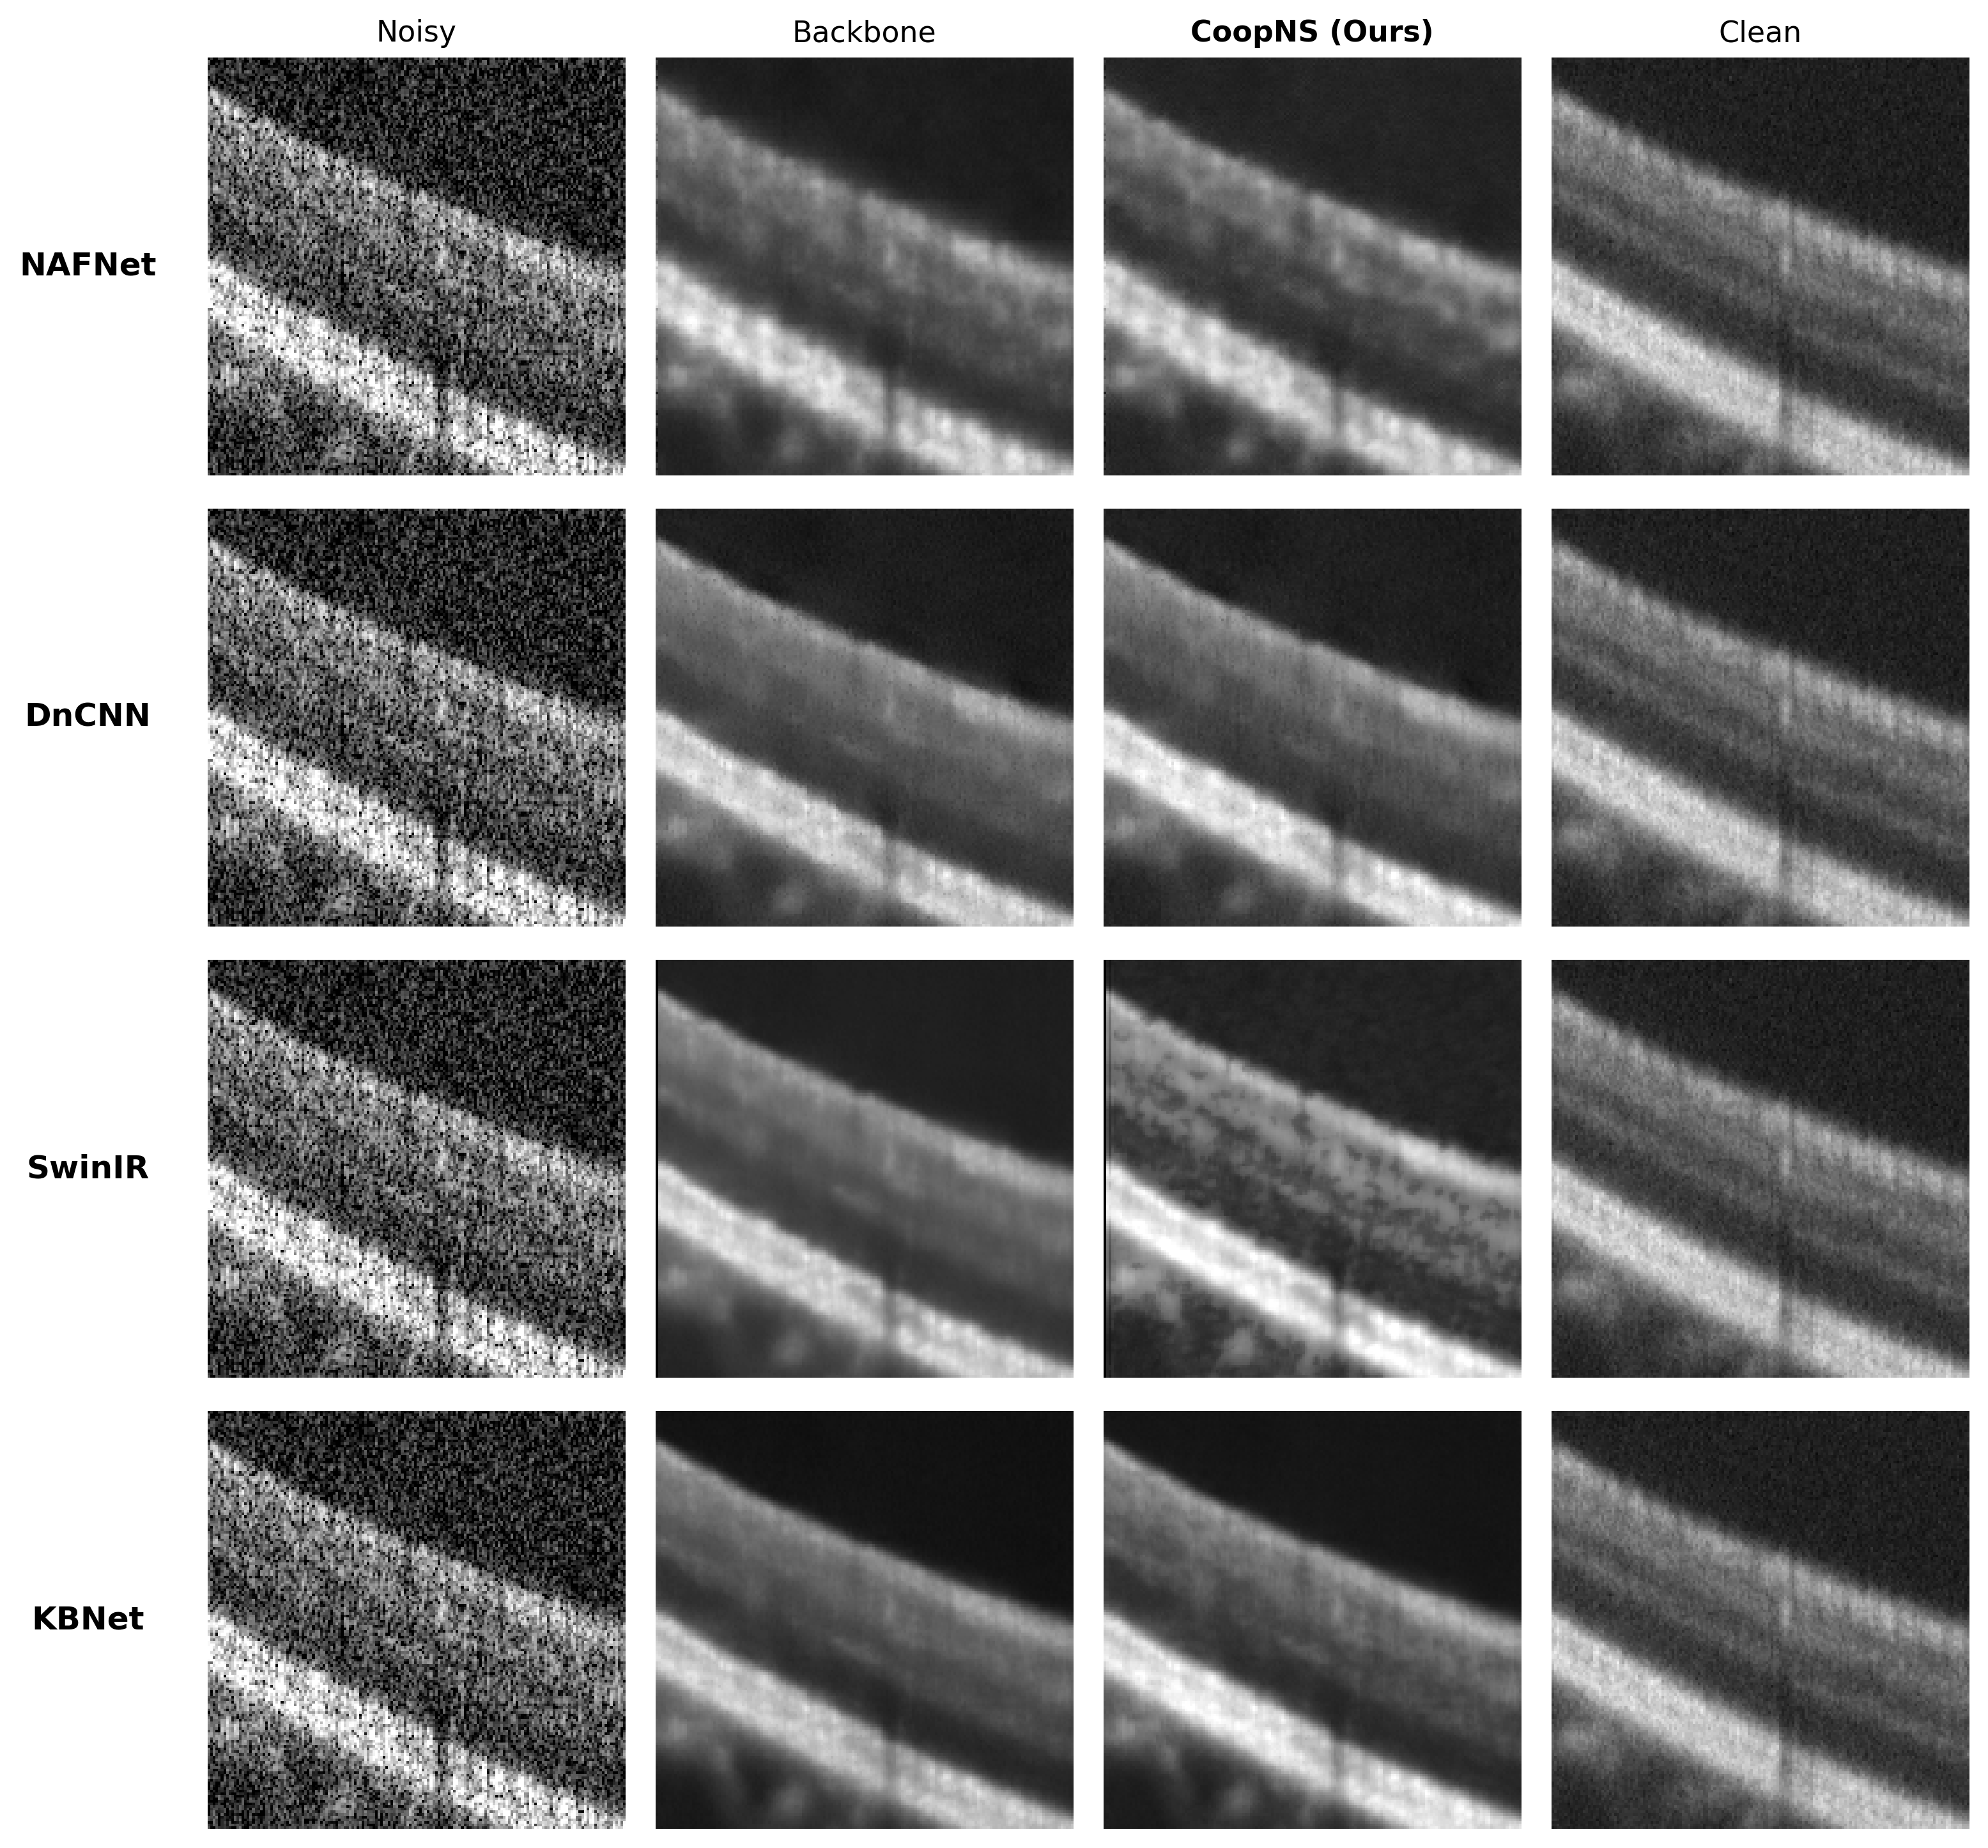
\includegraphics[width=0.84\textwidth]{figures/fig_subjective_pku37.png}
\caption{Subjective quality on PKU37 (in-distribution). Rows: NAFNet, DnCNN, SwinIR, KBNet. Columns: noisy input, backbone output, CoopNS-OCT-corrected output, clean reference. ROI crops use display range [0.15, 0.85] to reveal subtle boundary differences.}
\label{fig:subjective_pku37}
\end{figure*}

\begin{figure*}[t]
\centering
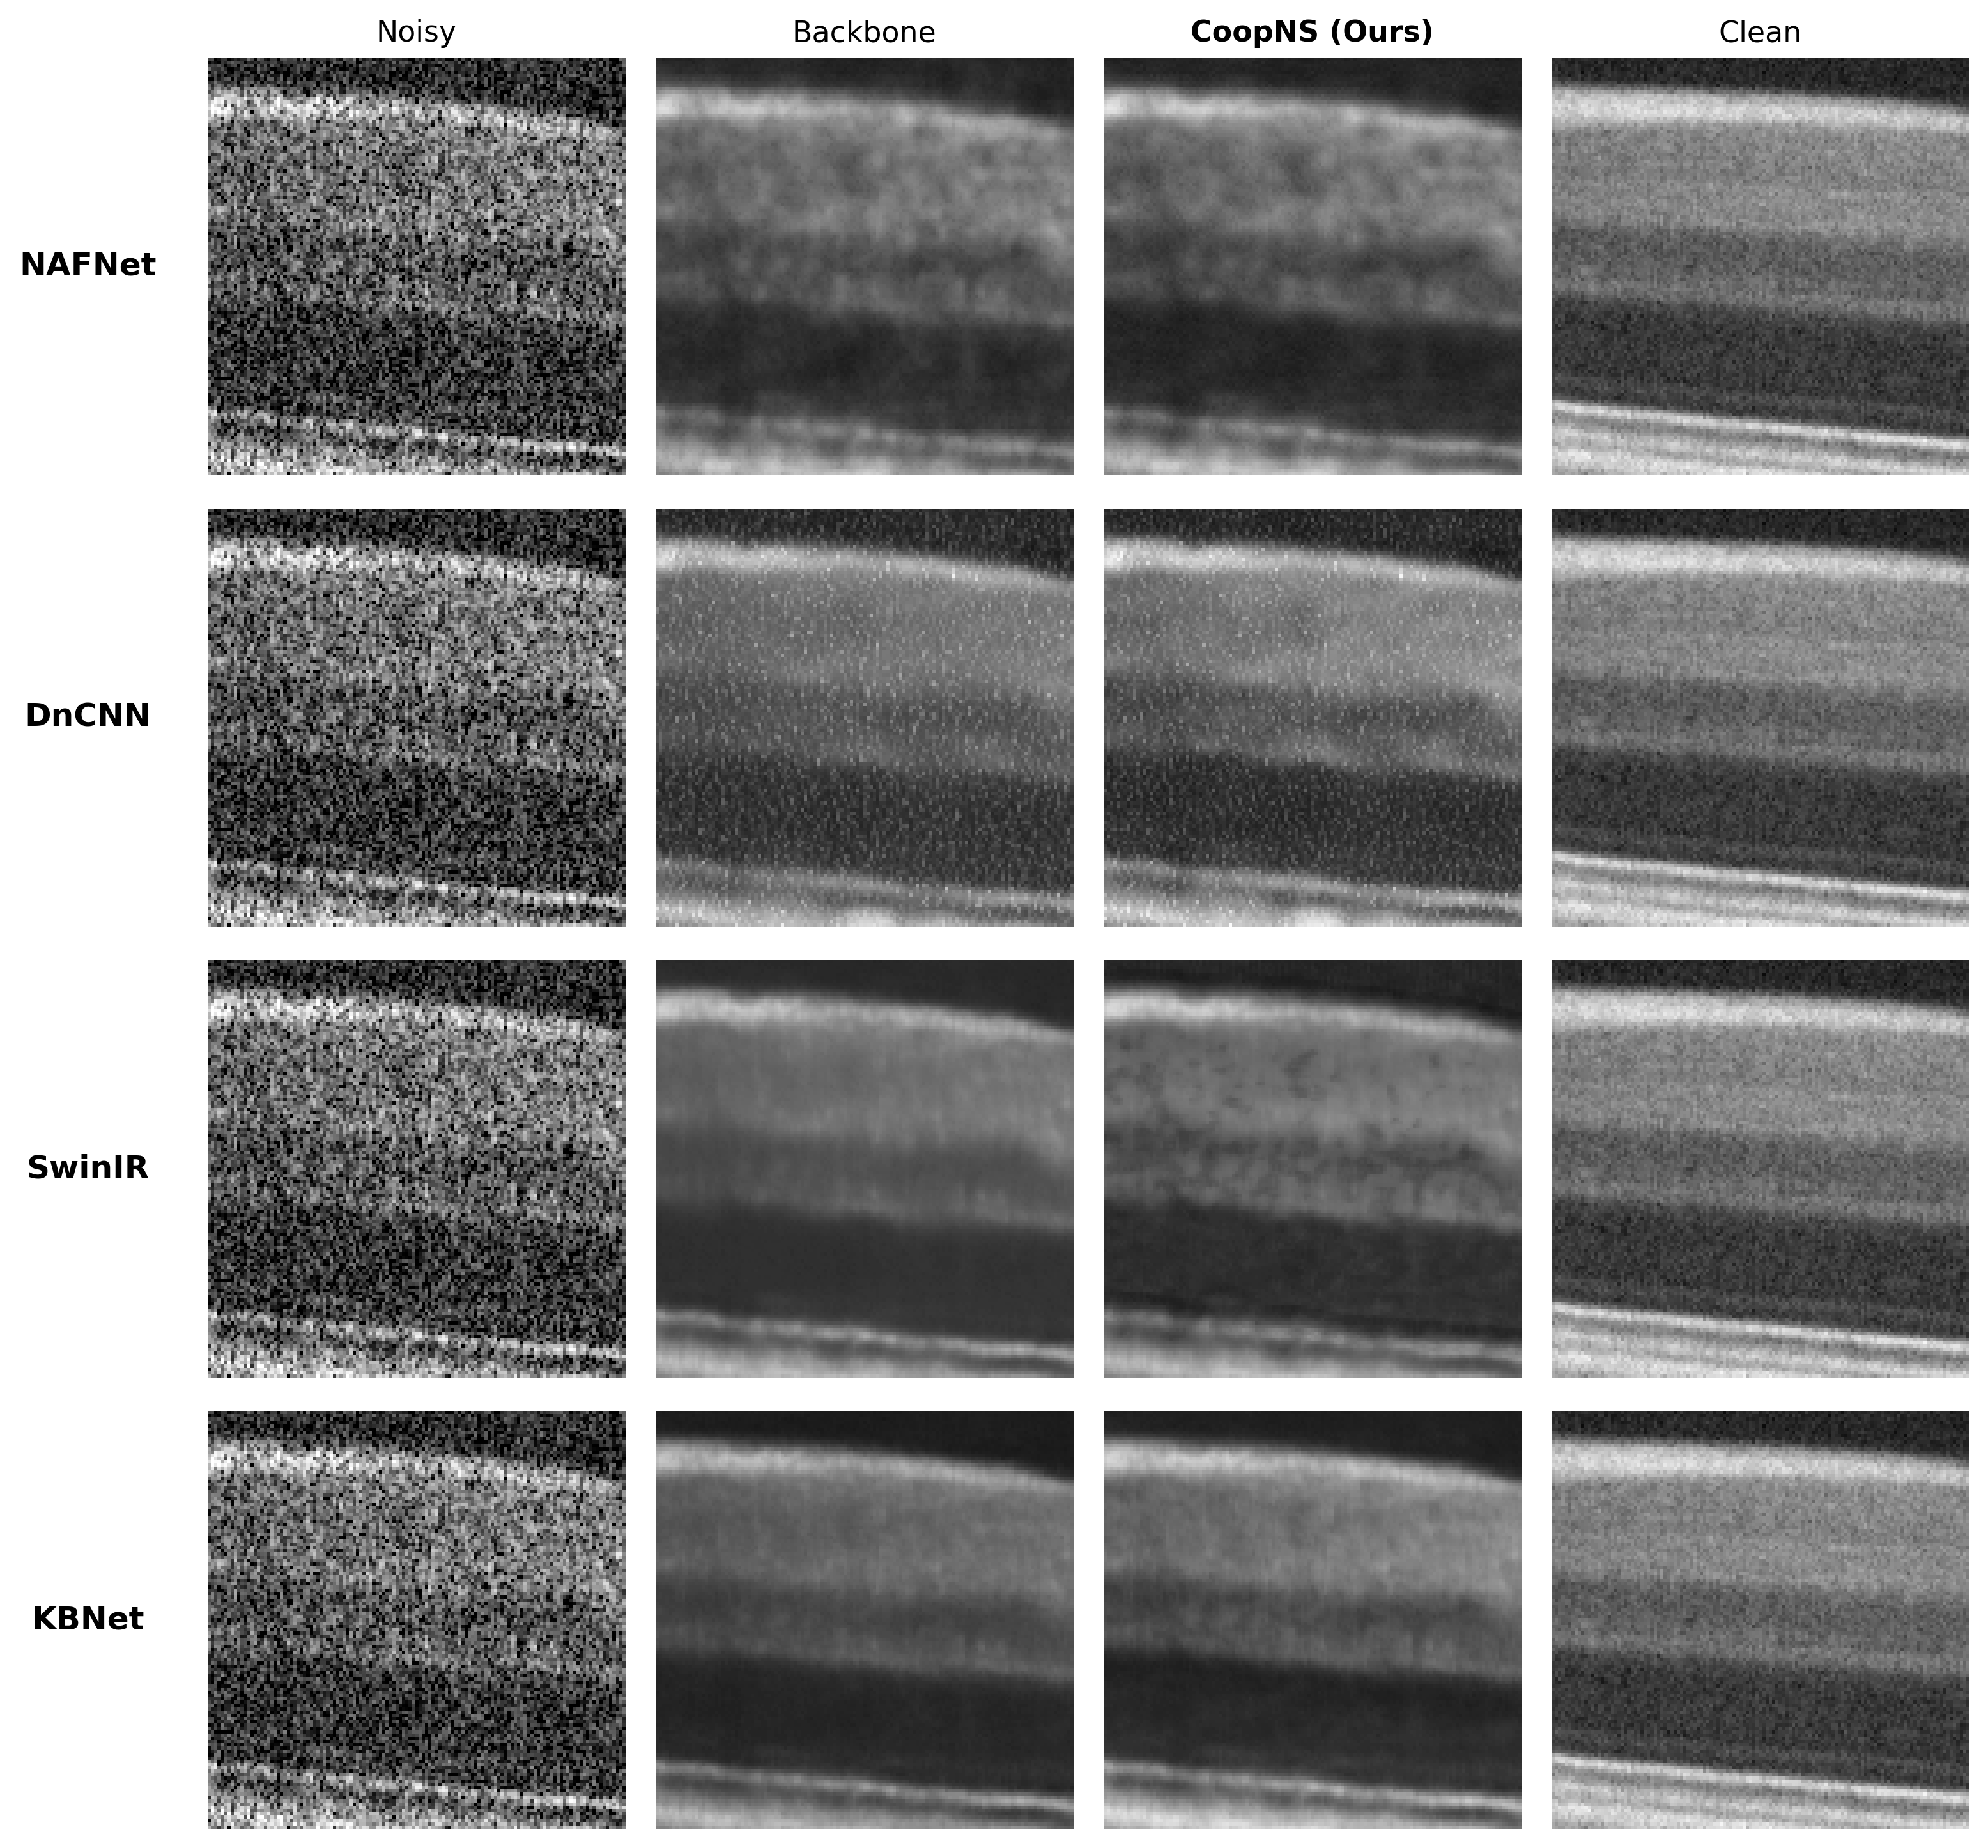
\includegraphics[width=0.84\textwidth]{figures/fig_subjective_duke17.png}
\caption{Subjective quality on Duke17 subject~9 (cross-dataset, LOO). Same layout as Fig.~\ref{fig:subjective_pku37}. CoopNS-OCT improves tissue--background contrast on out-of-distribution data from a different scanner, demonstrating cross-domain generalization.}
\label{fig:subjective_duke17}
\end{figure*}

\subsection{Cross-Dataset Generalization (LOO)}
\label{sec:results_ood}

We evaluate cross-scanner generalization via LOO cross-validation on Duke17~\cite{fang2012sparsity} (16 folds) and Duke2013~\cite{fang2013fast} (18 folds), training on $n{-}1$ images and testing on the held-out image with all four backbone families using the \emph{same} corrector architecture.

Table~\ref{tab:duke17_loo} reports LOO results on both cross-dataset benchmarks. Several observations merit discussion.

\textbf{Consistent CNR improvement.} All backbones achieve CNR gains of $+10$--$15\%$ on both benchmarks with controlled PSNR trade-off (-0.25 to -0.80\,dB), confirming cross-scanner generalization even though the corrector was trained exclusively on PKU37 data. The standard deviations across LOO folds are small relative to the mean improvements (e.g., CNR $\pm$ 2--4\% vs.\ means of $+10$--$15\%$), indicating stable corrections across subjects rather than memorized scanner-specific patterns.

\textbf{Complementary backbone profiles.} The corrector amplifies each backbone's distinct strengths. SwinIR+CoopNS-OCT achieves the highest TCI gains ($+38.9\%$ Duke17, $+25.5\%$ Duke2013), recovering tissue contrast suppressed by window-based self-attention during MSE training. DnCNN+CoopNS-OCT excels in noise suppression (ENL $+38.8\%$/$+37.8\%$) and edge recovery (EPI $+14.0\%$), while KBNet+CoopNS-OCT yields the strongest BS gains ($+6.7\%$/$+10.5\%$). DnCNN is also the only backbone with a consistent negative TCI shift on both OOD benchmarks ($-11.76\%$ and $-11.12\%$). This suggests that DnCNN already preserves intra-tissue dynamic range effectively under MSE training, and the multiplicative gain pathway trades some TCI for substantially improved ENL and EPI under symbolic control rather than uncontrolled regression.

\textbf{ID-to-OOD consistency.} CNR improvement narrows only slightly from the in-distribution range ($+9.7$--$15.1\%$) to the out-of-distribution range ($+10.2$--$15.1\%$), while PSNR trade-offs remain comparable. This indicates that the negotiated policy is not tied to a single scanner domain.

\textbf{Evaluation rigor.} The experimental design is intentionally stronger than a same-domain wrapper comparison. The corrector is trained once on PKU37, then transferred without redesign of the symbolic rules to two leave-one-out external benchmarks and four heterogeneous backbone families. The relevant baselines are therefore strong learned denoisers trained under the same protocol, while the ablation isolates the negotiator, edge recovery branch, and uncertainty guidance. The consistent gains across backbone replacement, dataset shift, and component removal are the main empirical evidence that the proposed object is not a fragile one-off combination.

\textbf{Generalization interpretation.} The corrector has only 0.168M trainable parameters and the symbolic rules depend on local contrast, edge, smoothness, speckle, and anatomical cues rather than scanner-specific metadata. The LOO results therefore support the claim that the wrapper captures transferable quality patterns rather than memorizing a single device domain.

\begin{table*}[t]
\centering
\caption{Cross-dataset generalization via leave-one-out cross-validation. Top: Duke17 (16 subjects); Bottom: Duke2013 (18 subjects). $\Delta$PSNR in dB; other metrics in $\Delta\%$.}
\label{tab:duke17_loo}
\resizebox{\textwidth}{!}{%
\begin{tabular}{lccccccc}
\toprule
& PSNR $\Delta$ (dB) & CNR $\Delta\%$ & TCI $\Delta\%$ & EPI $\Delta\%$ & BS $\Delta\%$ & ENL $\Delta\%$ & SNR $\Delta\%$ \\
\midrule
\multicolumn{8}{l}{\textit{Duke17 (16-fold LOO)}} \\
NAFNet + CoopNS-OCT & -0.40${\pm}$0.39 & $\mathbf{+10.27{\pm}2.13}$ & $\mathbf{+7.38{\pm}4.33}$ & $\mathbf{+1.88{\pm}0.75}$ & $\mathbf{+3.15{\pm}3.97}$ & +5.46${\pm}$16.27 & -3.16${\pm}$7.89 \\
KBNet + CoopNS-OCT & -0.39${\pm}$0.70 & $\mathbf{+12.05{\pm}1.92}$ & $\mathbf{+13.43{\pm}3.31}$ & -0.66${\pm}$0.60 & $\mathbf{+6.71{\pm}4.44}$ & $\mathbf{+12.72{\pm}10.99}$ & $\mathbf{+6.31{\pm}6.69}$ \\
DnCNN + CoopNS-OCT & -0.25${\pm}$0.41 & $\mathbf{+11.62{\pm}3.49}$ & -11.76${\pm}$4.45 & $\mathbf{+14.00{\pm}8.12}$ & +3.06${\pm}$7.36 & $\mathbf{+38.75{\pm}6.27}$ & $\mathbf{+18.28{\pm}4.06}$ \\
SwinIR + CoopNS-OCT & -0.71${\pm}$0.63 & $\mathbf{+10.20{\pm}3.65}$ & $\mathbf{+38.94{\pm}10.81}$ & $\mathbf{+3.61{\pm}3.61}$ & $\mathbf{+7.42{\pm}4.30}$ & $\mathbf{+11.95{\pm}14.50}$ & -3.12${\pm}$7.54 \\
\textit{Cross-backbone mean} & -0.44 & +11.02 & +12.00 & +4.71 & +5.09 & +17.22 & +4.58 \\
\midrule
\multicolumn{8}{l}{\textit{Duke2013 (18-fold LOO)}} \\
NAFNet + CoopNS-OCT & -0.47${\pm}$0.32 & $\mathbf{+12.86{\pm}2.58}$ & $\mathbf{+9.11{\pm}3.27}$ & $\mathbf{+1.44{\pm}1.43}$ & $\mathbf{+3.76{\pm}2.91}$ & +1.32${\pm}$15.19 & -5.59${\pm}$8.24 \\
KBNet + CoopNS-OCT & -0.42${\pm}$0.59 & $\mathbf{+13.47{\pm}2.13}$ & $\mathbf{+12.45{\pm}2.16}$ & -1.04${\pm}$0.34 & $\mathbf{+10.52{\pm}3.56}$ & $\mathbf{+12.90{\pm}7.29}$ & $\mathbf{+6.72{\pm}4.42}$ \\
DnCNN + CoopNS-OCT & -0.52${\pm}$0.38 & $\mathbf{+15.05{\pm}2.34}$ & -11.12${\pm}$6.59 & $\mathbf{+4.16{\pm}2.09}$ & $\mathbf{+2.55{\pm}3.80}$ & $\mathbf{+37.81{\pm}10.53}$ & $\mathbf{+14.74{\pm}5.47}$ \\
SwinIR + CoopNS-OCT & -0.80${\pm}$0.92 & $\mathbf{+11.79{\pm}2.99}$ & $\mathbf{+25.47{\pm}11.86}$ & $\mathbf{+3.55{\pm}1.95}$ & $\mathbf{+4.26{\pm}3.40}$ & $\mathbf{+18.03{\pm}12.04}$ & +0.61${\pm}$6.23 \\
\textit{Cross-backbone mean} & -0.55 & +13.29 & +8.98 & +2.03 & +5.27 & +17.52 & +4.12 \\
\bottomrule
\end{tabular}}
\end{table*}

\subsection{Ablation Study}
\label{sec:ablation}

We ablate the key components of CoopNS-OCT using the NAFNet backbone on the PKU37 test set (173~images). Table~\ref{tab:ablation} reports delta metrics relative to the backbone-only output.

\begin{table}[t]
\centering
\caption{Ablation study on PKU37 (NAFNet backbone). $\Delta$PSNR in dB; others in $\Delta\%$.}
\label{tab:ablation}
\setlength{\tabcolsep}{2.5pt}
\footnotesize
\begin{tabular}{lcccccc}
\toprule
Config. & $\Delta$PSNR & $\Delta$CNR & $\Delta$TCI & $\Delta$EPI & $\Delta$BS & $\Delta$ENL \\
\midrule
Full & -1.09 & +12.5 & +11.4 & +0.3 & +4.1 & +29.4 \\
w/o Negotiator & -1.01 & +10.8 & +13.5 & +0.3 & +4.1 & +4.6 \\
w/o Edge Rec. & -0.62 & +7.5 & +7.0 & +0.7 & +6.8 & +2.6 \\
w/o Uncert. & -0.94 & +13.5 & +8.6 & +0.7 & +3.2 & +27.4 \\
\bottomrule
\end{tabular}
\end{table}

\textbf{Edge recovery} is the most impactful component: removing it causes the largest drops in CNR ($+12.5 \to +7.5\%$) and ENL ($+29.4 \to +2.6\%$). Without additive edge corrections, the gain corrector attempts boundary restoration through multiplicative adjustments, which boosts EPI/BS but at the cost of substantially reduced speckle suppression. This confirms that separating boundary recovery (additive) from contrast enhancement (multiplicative) is architecturally important.

\textbf{The symbolic negotiator} primarily coordinates speckle suppression---without it, ENL drops from $+29.4\%$ to $+4.6\%$. TCI \emph{increases} slightly without the negotiator ($+13.5\%$ vs.\ $+11.4\%$) because unrestricted gain boosts contrast everywhere; the negotiator trades a small amount of raw contrast for substantially better speckle suppression.

\textbf{Uncertainty guidance} focuses corrections on structurally important regions; without it, corrections spread uniformly, yielding higher CNR ($+13.5\%$) but lower TCI ($+8.6\%$ vs.\ $+11.4\%$) and BS ($+3.2\%$ vs.\ $+4.1\%$). The higher CNR without uncertainty is misleading: uniform corrections inflate the CNR numerator at the cost of reduced tissue contrast and boundary sharpness.

No single ablation variant dominates across all metrics, confirming each component addresses a distinct aspect of the quality--fidelity balance.

%% =====================================================================
%% VII. DISCUSSION
%% =====================================================================
\section{Discussion}
\label{sec:discussion}

\textbf{Why this is more than a component combination.}
The paper does not argue that edge filters, confidence maps, or fuzzy operators are individually new. The claim is narrower and more technical: a clinically constrained OCT correction layer can be made \emph{explicit, stable, and transferable}. ``Explicit'' means closed-form predicate maps rather than hidden heuristics; ``stable'' means routing changes in a controlled way under predicate perturbations; ``transferable'' means the same policy remains usable after backbone replacement with only a localized interface change. That formal post-correction wrapper is the contribution being evaluated.

\textbf{Why the formalization matters technically.}
The explicit predicate maps are the interface that turns a qualitative clinical desideratum into a reproducible optimization target. Without them, the negotiator would consume hidden heuristics and the pipeline would collapse into an uninterpretable residual correction scheme.

\textbf{Why the modular claim is defensible.}
The confidence head is the only backbone-specific interface, and that dependency is deliberate. Different denoisers expose different feature dimensionalities and therefore require a small calibration adapter before uncertainty can be compared on a common scale. The rest of the wrapper---corrector branches, predicates, symbolic rules, and safety gates---is unchanged across NAFNet, DnCNN, SwinIR, and KBNet. The contribution is therefore not architecture-agnostic in the absolute sense, but modular in the stronger systems sense: the policy is shared, the adaptation cost is localized, and the empirical behavior remains stable after backbone replacement. Theorem~\ref{thm:allocation_stability} formalizes this point.

\textbf{Why the evaluation is sufficient for the claim being made.}
The paper does not claim a new state-of-the-art denoiser trained against every OCT restoration competitor. It claims a post-correction mechanism that should consistently add value to strong pretrained backbones under clinically motivated constraints. The relevant evidence is therefore backbone replacement, dataset shift, and targeted ablation.

\textbf{Why the safety layer matters operationally.}
The three constraints are not redundant. Energy descent controls aggregate clinical quality, the relaxed Pareto condition prevents one predicate from being improved by sacrificing several others, and bounded perturbation limits the magnitude of the image-level change itself. Together they make the wrapper easier to audit: one can inspect not only which predicates triggered correction, but also why a proposed correction was accepted only weakly or blended back toward the backbone output.

\textbf{Limitations.}
The bounded correction range means that the wrapper cannot fully repair severe backbone failures. The formal results are safety and transfer statements, not blanket performance guarantees: the stability theorem bounds routing sensitivity, and the CNR corollary gives a sufficient condition for non-decrease. Finally, the present submission is limited to the datasets and experiments already available in the repository; it does not include new reader studies or new simulations.
%% =====================================================================
%% VIII. CONCLUSION
%% =====================================================================
\section{Conclusion}
\label{sec:conclusion}

We presented CoopNS-OCT as a clinically constrained post-correction layer for OCT denoising rather than as a new denoising backbone. The contribution is a formal wrapper around pretrained denoisers: explicit mathematical definitions for the negotiator inputs, a stable neuro-symbolic allocation rule with a perturbation bound, and a safety-gated correction mechanism with a margin-based CNR guarantee. Across PKU37, Duke17 LOO, and Duke2013 LOO, the wrapper improves clinically relevant metrics with modest parameter overhead and controlled PSNR cost. The evidence supports a backbone-\emph{modular} conclusion: the same cooperative logic improves NAFNet, DnCNN, SwinIR, and KBNet after only adapting the confidence head.

Equally important, the paper makes the correction policy inspectable. Each clinical preference is exposed as an image-level predicate score and a spatial failure map, the symbolic negotiator converts those signals into a transparent allocation over corrector branches, and the final safety layer limits when and how strongly the corrected candidate can depart from the backbone output. That decomposition makes the framework reproducible and reusable: one can trace why a correction was proposed, where it was applied, and which constraint weakened or approved it, while still replacing the backbone and recalibrating only the confidence interface.


%% =====================================================================
%% REFERENCES
%% =====================================================================
{\small
\begin{thebibliography}{32}

\bibitem{huang1991optical}
D.~Huang, E.~A.~Swanson, C.~P.~Lin, J.~S.~Schuman, W.~G.~Stinson, W.~Chang, M.~R.~Hee, T.~Flotte, K.~Gregory, C.~A.~Puliafito, and J.~G.~Fujimoto, ``Optical coherence tomography,'' \emph{Science}, vol.~254, no.~5035, pp.~1178--1181, 1991.

\bibitem{goodman2007speckle}
J.~W.~Goodman, \emph{Speckle Phenomena in Optics: Theory and Applications}.\hskip 1em plus 0.5em minus 0.4em Roberts \& Company, 2007.

\bibitem{devalla2018drunet}
S.~K.~Devalla, P.~K.~Renukanand, B.~K.~Sreedhar, G.~Subramanian, L.~Zhang, S.~Perera, J.-M.~Mari, K.~S.~Chin, T.~A.~Tun, N.~G.~Strouthidis, and M.~J.~A.~Girard, ``DRUNET: A dilated-residual U-Net deep learning network to segment optic nerve head tissues in optical coherence tomography images,'' \emph{Biomed.\ Opt.\ Express}, vol.~9, no.~7, pp.~3244--3265, 2018.

\bibitem{zhang2017beyond}
K.~Zhang, W.~Zuo, Y.~Chen, D.~Meng, and L.~Zhang, ``Beyond a Gaussian denoiser: Residual learning of deep CNN for image denoising,'' \emph{IEEE Trans.\ Image Process.}, vol.~26, no.~7, pp.~3142--3155, 2017.

\bibitem{chen2022simple}
L.~Chen, X.~Chu, X.~Zhang, and J.~Sun, ``Simple baselines for image restoration,'' in \emph{Proc.\ ECCV}, 2022, pp.~17--33.

\bibitem{liang2021swinir}
J.~Liang, J.~Cao, G.~Sun, K.~Zhang, L.~Van~Gool, and R.~Timofte, ``SwinIR: Image restoration using Swin Transformer,'' in \emph{Proc.\ ICCV Workshops}, 2021, pp.~1833--1844.

\bibitem{krull2019noise2void}
A.~Krull, T.-O.~Buchholz, and F.~Jug, ``Noise2Void---learning denoising from single noisy images,'' in \emph{Proc.\ CVPR}, 2019, pp.~2129--2137.

\bibitem{rodriguez2020generalized}
A.~Rodriguez-Molares, O.~M.~H.~Rindal, J.~D'hooge, S.-E.~Masoy, A.~Austeng, M.~A.~Lediju~Bell, and H.~Torp, ``The generalized contrast-to-noise ratio: A formal definition for lesion detectability,'' \emph{IEEE Trans.\ Ultrason., Ferroelectr., Freq.\ Control}, vol.~67, no.~4, pp.~745--759, 2020.

\bibitem{defauw2018clinical}
J.~De~Fauw, J.~R.~Ledsam, B.~Romera-Paredes, \emph{et~al.}, ``Clinically applicable deep learning for diagnosis and referral in retinal disease,'' \emph{Nature Med.}, vol.~24, pp.~1342--1350, 2018.

\bibitem{vankrieken2022analyzing}
E.~van~Krieken, E.~Acar, and F.~van~Harmelen, ``Analyzing differentiable fuzzy logic operators,'' \emph{Artif.\ Intell.}, vol.~302, art.~103602, 2022.

\bibitem{zhang2023kbnet}
Y.~Zhang, D.~Li, X.~Shi, D.~He, K.~Song, X.~Wang, H.~Qin, and H.~Li, ``KBNet: Kernel basis network for image restoration,'' Tech.\ Rep.\ arXiv:2303.02881, 2023. [Online]. Available: \url{https://arxiv.org/abs/2303.02881}

\bibitem{buades2005non}
A.~Buades, B.~Coll, and J.-M.~Morel, ``A non-local algorithm for image denoising,'' in \emph{Proc.\ CVPR}, vol.~2, 2005, pp.~60--65.

\bibitem{mayer2012wavelet}
M.~A.~Mayer, A.~Borsdorf, M.~Wagner, J.~Hornegger, C.~Y.~Mardin, and R.~P.~Tornow, ``Wavelet denoising of multiframe optical coherence tomography data,'' \emph{Biomed.\ Opt.\ Express}, vol.~3, no.~3, pp.~572--589, 2012.

\bibitem{geng2022triplet}
M.~Geng, X.~Meng, L.~Zhu, Z.~Jiang, M.~Gao, Z.~Huang, B.~Qiu, Y.~Hu, Y.~Zhang, Q.~Ren, and Y.~Lu, ``Triplet cross-fusion learning for unpaired image denoising in optical coherence tomography,'' \emph{IEEE Trans.\ Med.\ Imag.}, vol.~41, no.~11, pp.~3357--3372, 2022.

\bibitem{fang2012sparsity}
L.~Fang, S.~Li, Q.~Nie, J.~A.~Izatt, C.~A.~Toth, and S.~Farsiu, ``Sparsity based denoising of spectral domain optical coherence tomography images,'' \emph{Biomed.\ Opt.\ Express}, vol.~3, no.~5, pp.~927--942, 2012.

\bibitem{fang2013fast}
L.~Fang, S.~Li, R.~P.~McNabb, Q.~Nie, A.~N.~Kuo, C.~A.~Toth, J.A.~Izatt, and S.~Farsiu, ``Fast acquisition and reconstruction of optical coherence tomography images via sparse representation,'' \emph{IEEE Trans.\ Med.\ Imag.}, vol.~32, no.~11, pp.~2034--2049, 2013.

\bibitem{wang2019quality}
J.~Wang, G.~Deng, W.~Li, Y.~Chen, F.~Gao, H.~Liu, Y.~He, and G.~Shi, ``Deep learning for quality assessment of retinal OCT images,'' \emph{Biomed.\ Opt.\ Express}, vol.~10, no.~12, pp.~6057--6072, 2019.

\bibitem{gal2016dropout}
Y.~Gal and Z.~Ghahramani, ``Dropout as a Bayesian approximation: Representing model uncertainty in deep learning,'' in \emph{Proc.\ ICML}, 2016, pp.~1050--1059.

\bibitem{kendall2018multi}
A.~Kendall, Y.~Gal, and R.~Cipolla, ``Multi-task learning using uncertainty to weigh losses for scene geometry and semantics,'' in \emph{Proc.\ CVPR}, 2018, pp.~7482--7491.

\bibitem{lakshminarayanan2017simple}
B.~Lakshminarayanan, A.~Pritzel, and C.~Blundell, ``Simple and scalable predictive uncertainty estimation using deep ensembles,'' in \emph{Proc.\ NeurIPS}, 2017, pp.~6402--6413.

\bibitem{garcez2023neurosymbolic}
A.~d'Avila~Garcez and L.~C.~Lamb, ``Neurosymbolic AI: The 3rd wave,'' \emph{Artif.\ Intell.\ Rev.}, vol.~56, pp.~12387--12406, 2023.

\bibitem{fdaaiml2021}
U.S.\ Food and Drug Administration, ``Artificial intelligence/machine learning (AI/ML)-based software as a medical device (SaMD) action plan,'' FDA, Jan.\ 2021.

\bibitem{stein2006quality}
D.~M.~Stein, H.~Ishikawa, R.~Hariprasad, G.~Wollstein, R.~J.~Noecker, J.~G.~Fujimoto, and J.~S.~Schuman, ``A new quality assessment parameter for optical coherence tomography,'' \emph{Br.\ J.\ Ophthalmol.}, vol.~90, no.~2, pp.~186--190, 2006.

\bibitem{tewarie2012oscar}
P.~Tewarie, L.~Balk, F.~Costello, A.~Green, R.~Martin, S.~Schippling, and A.~Petzold, ``The OSCAR-IB consensus criteria for retinal OCT quality assessment,'' \emph{PLoS ONE}, vol.~7, no.~4, art.~e34823, 2012.

\bibitem{kingma2015adam}
D.~P.~Kingma and J.~Ba, ``Adam: A method for stochastic optimization,'' in \emph{Proc.\ ICLR}, 2015.

\bibitem{wang2004image}
Z.~Wang, A.~C.~Bovik, H.~R.~Sheikh, and E.~P.~Simoncelli, ``Image quality assessment: From error visibility to structural similarity,'' \emph{IEEE Trans.\ Image Process.}, vol.~13, no.~4, pp.~600--612, 2004.

\bibitem{loshchilov2019decoupled}
I.~Loshchilov and F.~Hutter, ``Decoupled weight decay regularization,'' in \emph{Proc.\ ICLR}, 2019.

\bibitem{gonzalez2018digital}
R.~C.~Gonzalez and R.~E.~Woods, \emph{Digital Image Processing}, 4th~ed.\hskip 1em plus 0.5em minus 0.4em Pearson, 2018.

\bibitem{cohen1988statistical}
J.~Cohen, \emph{Statistical Power Analysis for the Behavioral Sciences}, 2nd~ed.\hskip 1em plus 0.5em minus 0.4em Lawrence Erlbaum Associates, 1988.

\end{thebibliography}
}

\end{document}
